% !TEX root = ../../../main.tex
% 来源：中学数学实验教材·第三册（高中数学）
% 章节：不等式和解不等式 / 大小次序与不等式
% 原始文件：3.tex，行 458-468
% 类型：tikz
% ---
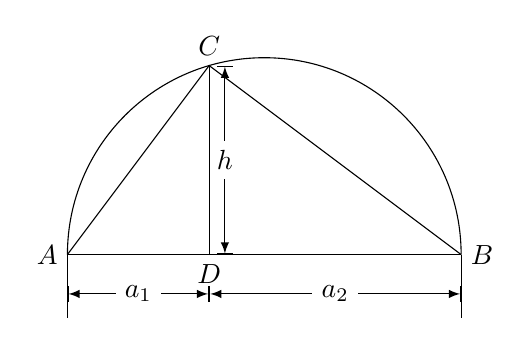
\begin{tikzpicture}[>=latex]
    \draw[|<->|] (2,0)--node[fill=white]{$h$}(2,2.4);
 \draw (0,0)node[left]{$A$}--(5,0)node[right]{$B$};
\draw (5,0) arc (0:180:2.5);    
\draw (1.8,2.4)node[above]{$C$}--(1.8,0)node[below]{$D$};
\draw (0,0)--(1.8,2.4)--(5,0);
\draw[|<->|] (0,-.5)--node[fill=white]{$a_1$}(1.8,-.5);
\draw[|<->|] (5,-.5)--node[fill=white]{$a_2$}(1.8,-.5);
\draw (0,0)--(0,-.8);\draw (5,0)--(5,-.8);

\end{tikzpicture} 
